\documentclass[9pt,twocolumn,twoside,lineno]{pnas-new}
% Use the lineno option to display guide line numbers if required.
% Note that the use of elements such as single-column equations
% may affect the guide line number alignment. 

\templatetype{pnasresearcharticle} % Choose template 
% {pnasresearcharticle} = Template for a two-column research article
% {pnasmathematics} = Template for a one-column mathematics article
% {pnasinvited} = Template for a PNAS invited submission
\usepackage{amssymb,amsfonts,amsthm,bm}
\usepackage{adjustbox}
\usepackage[round,numbers,sort&compress]{natbib}
\usepackage{graphicx}
\usepackage{amssymb}
\usepackage{fixltx2e}
\usepackage{graphicx}
\usepackage{wrapfig, blindtext}
\usepackage{setspace} 
\usepackage{caption}
%\usepackage{subcaption}
%\usepackage{subfig}
%\usepackage[ansinew]{inputenc}
%\usepackage{xspace}

\begin{document}
\title{Cross-pore electrostatic repulsions are critical for stabilizing the GABA\textsubscript{A} receptor open state}

\author[a,1]{Sruthi Murlidaran}
\author[a,b,2]{Reza Salari}
\author[a,b,3]{Grace Brannigan}

\affil[a]{Rutgers University, Center for Computational and Integrative Biology, Rutgers University, Camden, NJ, USA}
\affil[b]{Department of Physics, Rutgers University, Camden, NJ, USA}

\newcommand{\GABAA}{GABA\textsubscript{A}R\xspace}
\newcommand{\avgr}{\bar{r}}
\newcommand{\varr}{\delta r^{2}}
\newcommand{\plgics}{pLGICs}
\newcommand{\nachr}{nAChR}
%%


%\newcommand{\GABAA}{GABA\textsubscript{A}R\xspace}
%\newcommand{\avgr}{\bar{r}}
%\newcommand{\varr}{\delta r^{2}}
%\newcommand{\plgics}{pLGICs}
%\newcommand{\nachr}{nAChR}
\begin{abstract}
{GABA\textsubscript{A} receptors (\GABAA) are critical for proper transmission of inhibitory signals in the central nervous system, and are common targets of anesthetic and anxiolytic drugs.  Several naturally occurring mutations in such receptors can cause an increased likelihood of seizures. In particular, gamma-K289M on the M2-M3 loop attached to the pore-lining M2 helices is associated with Generalized Epilepsy and Febrile Seizures.   At the single channel level, the mutation dramatically reduces current amplitude in some subspecies, and increases deactivation rate in other subspecies.  The molecular mechanism through which the mutation causes these effects is unknown.  Using a homology model of the \GABAA  based on the recently solved structure for the homologous glutamate-gated chloride channel (GluCl), we ran molecular dynamics simulations  of multiple replicas incorporating both the Wild-type and the mutation, at room temperature and at temperatures inducing febrile seizures. These simulations have shown distinct effects on conformations and conductance of the channel. From these results we propose a molecular mechanism for rapid but unstable closure of \GABAA, which would be likely to cause flickering effect reported by experimental studies, in single channel recordings.}
\end{abstract}

%%%%%%%%%%%%%%%%%%%%%%%%%%%%%%%%%%%%%%%%%%%%%%%%%%%%%%%%%%%%%%%%%%%%%
%% Start the main part of the manuscript here.
%%%%%%%%%%%%%%%%%%%%%%%%%%%%%%%%%%%%%%%%%%%%%%%%%%%%%%%%%%%%%%%%%%%%%
\maketitle
\thispagestyle{firststyle}
\ifthenelse{\boolean{shortarticle}}{\ifthenelse{\boolean{singlecolumn}}{\abscontentformatted}{\abscontent}}{}


%\markboth{Dedecker et al.}{Fast and Reversible Photoswitching}

\section*{INTRODUCTION}

\newcommand{\WT}{WT\xspace}
\newcommand{\MT}{K289M\xspace}
\newcommand{\RMSD}{RMSD\textsubscript{symm}\xspace}
\newcommand{\WTs}{WT systems\xspace}
\newcommand{\MTs}{K289M systems\xspace}
\newcommand{\RMSDs}{RMSDs\textsubscript{symm}\xspace}
%\newcommand{C} {Cl\textsubscript{-}\xspace}
%\newcommand{\GABAA}{\emph GABA\textsubscript{A}R\xspace}

  Pentameric Ligand-gated Ion Channels (pLGICs) are essential components of the post-synaptic membrane, serving both inhibitory and excitatory roles.  pLGIC sequence varies significantly within and between prokaryotes and eukaryotes,\cite{Jaiteh2016} with typical homologies of about 30\%.  pLGIC function tends to be quite sensitive to even small differences in sequence, but numerous pLGIC structures have now demonstrated significant structural conservation despite functional variation.  This property has made it challenging to isolate the roles of various pLGIC components or sequence variations in subtle functional effects.  
    
  Despite the high sequence variation among pLGIC subunits, even for those forming a heteromeric channel, few single nucleotide polymorphisms (SNPs) are found among populations within coding regions for a specific subunit.   Mutations causing loss of function in inhibitory receptors or gain of function in excitatory receptors can result in seizures induced by neuron overexcitation. Many naturally occurring mutations are associated with various forms of epilepsy\cite{Bianchi2002,Cossette2002,Kang2004,Macdonald2004}, with several relevant mutations identified even before the use of genome-wide association studies. The molecular mechanisms underlying the effect of nearly all mutations on signaling are unknown.

GABA is the primary inhibitory neurotransmitter in the central nervous system; inhibition is partially transduced by extracellular binding to the type A GABA receptor, an anionic pLGIC\cite{Olsen1990,Macdonald1994,Rabow1995}. Many molecules with sedative, anxiolytic, and anesthetic properties are positive modulators of the \GABAA, including neurosteroids\cite {Mihic1997,Belelli2005a, Mitchell2008,Lambert2009,Olsen2011a}, benzodiazepines\cite{Sigel1997}, and inhalational and intravenous general anesthetics\cite {Krasowski1999,Harris1995,Miller2002}. Negative modulators, such as pregnenolone sulfate\cite{Majewska1988}, can induce seizures, as can certain mutations. Seizures associated with inherited mutations typically require conditions that are found only infrequently; survival is unlikely in the presence of consistent seizures.  \GABAA receptors with these mutations are therefore known a priori to be functional under typical conditions but dysfunctional under well-defined alternate conditions, making them promising candidates for identifying the role of the mutated residue.   

Each subunit consists of an extracellular agonist-binding domain (ECD) and a transmembrane domain containing a four helix bundle with helices labeled (M1-M4).  The M2 helices line the pore, and the M2-M3 loop connecting the M2 and M3 helices interacts directly with the ECD.  The loop has long been hypothesized to ``communicate'' agonist binding to the transmembrane domain,\cite{Campos-Caro1996,Lynch1997,Grosman2000,Bera2002,Lummis2005,Law2005,Lee2005,Unwin2005, Lee2009} with several mutation studies indicating the importance for agonist sensitivity of short-range attractive electrostatic interactions, such as salt-bridges, between the M2-M3 loop and the ECD. \cite{Sigel1999, OShea2000, Kash2003, Hales2006} 

In \GABAA subunits the M2-M3 loop contains a basic residue appearing at the homologous positions of $\alpha279, \beta274,$ or $\gamma289$, notated as M2 24$^{\prime}$ in the prime numbering scheme suggested in \cite{Jaiteh2016}.  Harrison and colleagues\cite{Kash2003} demonstrated that charge-reversal of $\alpha279$ reduced agonist sensitivity (EC50) which was restorable via additional charge-reversal of $\alpha$ D57 or $\alpha$D149, both within the ECD and expected to be near the M2-M3 loop.  Maximum whole-cell current, however, was reduced by about 1/3 upon the single $\alpha D279K$ mutation, and further reduced by about the same amount with the second mutation of $\alpha$ D57K or $\alpha$D149K, suggesting a significant role for $\alpha279K$ in stabilizing the open state beyond forming a salt-bridge with the ECD.  Similar behavior was observed in the nicotinic acetylcholine receptor (\nachr), upon charge-reversal of  $\alpha$ R209 in M1 and $\alpha$ E45 in the ECD.\cite{Lee2005}  

A natural but uncommonly occurring SNP at the homologous residue in the $\gamma$ subunit ($\gamma2$ K289), further suggests an additional role for this residue beyond gating, because the $\gamma$ subunit does not form GABA binding cavities. The \(\gamma\)\textsubscript{2}:K289M mutation has been reported in families with generalized epilepsy and febrile seizures plus(GEFS+)\cite{Mac2010,Baulac2001,Bianchi2002}, a generalized phenotype that often includes only febrile (fever-caused) seizures until about age 11, but can also include less severe myoclonic, atonic, or absence seizures at normal body temperature.  In \(\alpha\)\textsubscript{1}\(\beta\)\textsubscript{2}\(\gamma\)\textsubscript{2} K289M receptors, GABA-evoked current amplitude was dramatically reduced relative to the \WT \cite{Baulac2001,Ramakrishnan2004}, while in \(\alpha\)\textsubscript{1}\(\beta\)\textsubscript{3}\(\gamma\)\textsubscript{2}K289M receptors the mutation did not affect current amplitudes but did increase the deactivation rate\cite{Eugene2007}. In the latter receptors, currents had reduced mean open times, in part due to flickering\cite{Bianchi2002,Macdonald2006,Hales2006}. In hippocampal neurons containing \GABAA with \(\gamma\)\textsubscript{2}:K289M subunits %and ratios of subtypes for \(\alpha\) and \(\beta\) subunits left relatively unaffected, 
accelerated deactivation of inhibitory post synaptic currents was also observed\cite{Eugene2007}.

%pLGICs are heteromers: each subunit consists of an extracellular domain (ECD) composed of beta sandwiches and a four helix bundle comprising the transmembrane domain (TMD).
%%\cite{Corringer2012}. 
%Many eukaryotic pLGICs also contain an intracellular domain, for which little structural information is available, but which is not required for function.  \cite{Jansen2008}. 
%Due to a highly conserved disulfide bridge found on a loop in the ECD in many eukaryotic pLGICs, receptors in this class are also termed Cys-loop receptors, although prokaryotic homologs identified thus far do not contain the disulfide bridge\cite{Sine2006,Mieke2013,Hilf2009a,Bocquet2009,Nury2011,Spurny2013}.
%
%Several pLGICs exhibit significant subunit diversity, particularly \GABAA. Thus far, 19 \GABAA subunits have been identified, labeled (\(\alpha\)1-\(\alpha\)6, \(\beta\)1-\(\beta\)3, \(\gamma\)1- \(\gamma\)3, \(\delta\), \(\epsilon\), \(\theta\) and \(\rho\)1-\(\rho\)3)\cite{Sieghart1995,Schofield1987,Davies1997,Hedblom1997,Bonnert1999}. The most commonly found \GABAA stoichiometry in the human brain is \(\alpha\)1\(\beta\)2\(\gamma\)2, which is arranged \(\alpha\)1-\(\beta\)2-\(\alpha\)1-\(\beta\)2-\(\gamma\)2 clockwise around a central pore as shown in \cite{cworder}. GABA binds to the interface between \(\alpha\) and \(\beta\) subunits, in the ECD, causing activation of the channel through a mechanism that is only partially understood\cite{Farrar1999,Sieg2002,Mieke2013}.
%
% Medium resolution structures from cryo Electron Microscopy of nAChRs\cite{Miyazawa2003,Unwin2005} provided early insights into fundamental structural elements, demonstrating that the transmembrane domain of pLGICs consists of four membrane spanning \(\alpha\)-helices (M1-M4), with M2 as the the pore lining helix; the extensive intracellular domain found in \GABAA lies between M3 and M4.  M2 and M3 helices are separated by a short loop termed the M2-M3 loop, which directly contacts the ECD and has been suggested as an essential component of the activation process\cite{Campos-Caro1996,Lynch1997,Grosman2000,Bera2002,Lummis2005,Law2005} by coupling agonist binding to channel gating.\cite{Lee2005,Lee2009}. In particular, formation of a salt bridge between Lys279 in the \(\alpha\)\textsubscript{1} subunit and Asp149 in the extracellular loop during gating has been observed in the \GABAA\cite{Kash2003}.Further, single point mutation studies of the Lys\cite{Sigel1999,Hales2006} and Arg\cite{OShea2000} residues in the M2-M3 linker of  \(\alpha\)\textsubscript{1}\(\beta\)\textsubscript{1} subunits have been shown to affect gating by GABA.
 
% Recently, a homo \(\beta\)3 pentamer has been crystalized to a 3\AA\ resolution\cite{Miller2014}. High resolution structures are also available for a eukaryotic, anion-selective homolog, the glutamate-gated chloride channel (GluCl),from C Elegans\cite{Hibbs2011a,glucl-lipid}, and the glycine receptor\cite{glyr} as well as the cationic nicotinic acetylcholine receptor and 5HT-3 receptors well as several structures for the prokaryotic cationic homologs, GLIC\cite{Hilf2009a, Bocquet2009, Sauguet2013} and ELIC\cite{Hilf2008,Pan2012,Spurny2012}.

%Several mutations of \GABAA are naturally found in human populations and are associated with various seizure disorders\cite{Mac2010}, including \(\alpha\)\textsubscript{1}:A322D\cite{Krampfl2005}, \(\delta\):E177A\cite{Feng2006}, \(\delta\):R220H \cite{Feng2006} , \(\gamma\)\textsubscript{2}:R43Q\cite{Kang2004,Hales2005}, and \(\gamma\)\textsubscript{2}:K289M\cite{Baulac2001,Bianchi2002}. The present paper focuses on effects of the \(\gamma\)\textsubscript{2}:K289M mutation, which has been reported in families with generalized epilepsy and febrile seizures (FS)\cite{Mac2010,Baulac2001,Bianchi2002}. Lys 289 , located in the M2-M3 loop of the \(\gamma\)\textsubscript{2} subunit has been associated with several potential effects upon mutation. 
%%Previous paragraph rewritten-26FEB%
%Initially reduced activity of GABAa receptor was implicated with epilepsy following which several mutations of GABA\textsubscript{A} receptors that are naturally found in human populations\citeMacdonald2004 were associated with various seizure disorders\cite{Mac2010}, including \(\alpha\)\textsubscript{1}:A322D\cite{Cossette2002}, \(\delta\):E177A\cite{Feng2006}, \(\delta\):R220H \cite{Feng2006} , \(\gamma\)\textsubscript{2}:R43Q\cite{Wallace2001}, and \(\gamma\)\textsubscript{2}:K289M\cite{Baulac2001}. The present paper focuses on effects of the \(\gamma\)\textsubscript{2}:K289M mutation,which has been reported in families with generalized epilepsy and febrile seizures (FS)\cite{Baulac2001}. 

 %%Lys 289,located in the M2-M3 loop,is a conserved residue in various subunits of GABA\textsubscript{A} receptor and orthologous subunits of other cys-loop receptors{Baulac2001}.The K289M mutation in the  \(\gamma\)\textsubscript{2} subunit is associated with several potential effects upon mutation. Though the mutation was initially thought to  dimnish the current amplitude\cite{Baulac2001,Ramakrishnana2004}, increasing evidence have suggested that the the mutation accelerates deactivation rate caused due to reduced mean channel opening time\cite{Bianchi2002,Hales2006,Eugene2007,O'Mara2005}

%K289M, also associated with FS has been shown to cause temperature-dependent effects on membrane expression, trafficking \cite{Kang2006},membrane dynamics and receptor kinetics\cite{Bouthour2012}. It has been observed that, membrane trafficking was more temperature dependent with receptors containing mutations in \(\gamma\)\textsubscript{2} subunits, than in other subunits\cite{Kang2006}. Further, temperature induced decrease in frequency of mIPSCs was associated with depletion of mutation containing post-synaptic receptors\cite{Bouthour2012}.
%Due to the proximity of the mutation to the pore and gating apparatus of the \GABAA, mechanisms resulting from effects on conductance and gating kinetics at the single channel level remain the most direct of those proposed.

Little information has been available regarding the effect of the mutation on \GABAA structure and dynamics. Using a homology model of the \GABAA receptor based on the medium resolution cryo electron microscopy structure of the nicotinic Acetylcholine Receptor (nAChR), Brownian Dynamics Simulations of ion conduction were used to suggest that mutant receptors display reduced conductance due to reduced affinity of the ion for the ion channel\cite{O'Mara2005}. However, the recent x-ray structures of eukaryotic and prokaryotic homologs have suggested that alignment of the sequence with the electron density map in the M2 helices is likely incorrect in the structure used for these simulations. Furthermore, these simulations do not contain explicit representations of water or lipid molecules.

The temperature dependence of this mutation suggests a significant role for  entropy and conformational fluctuations in determining its effects.  Here we conduct molecular dynamics simulations with multiple replicas of the $\gamma$2 K289 and M289 forms of the receptor, at both lower and higher temperatures.  We observe a moderately narrowed pore in the M289 receptor at 300K, and a significantly narrowed pore at 315K.  Through adaptive biasing force (ABF) calculations, we demonstrate that the effects at 315K result in a substantially higher barrier for conduction of a chloride ion.  

$\gamma2$ K289 was not observed to form salt bridges with the ECD, and these conformational effects showed no clear correlation to any salt-bridging pattern.  We propose instead that the five conserved basic residues at this position form a ring of positive charge that effectively pushes the five M2-M3 loops away from the center, pulling M2 helices with it, and stabilizing the open state.   Neutralizing one of the charges as with $\gamma_{2}K289M$ reduces this repulsion.  When it is combined with a temperature increase that softens the conformational preferences resulting from remaining interactions common to both K and M receptors, the non-temperature dependent change in electrostatic repulsions dominates.  

We present a simple variational theory that quantitatively predicts the effect of $\gamma_{}$2:K289M on the preferred separation of M2-M3 loop charges, using only the mean and standard deviation of the separation in the wild type $\gamma_{}2$:K289 channel. Temperature dependence appears through both the effect of temperature on the standard deviation and as a linear term in the theory.  The success of the theory supports a critical role for these electrostatic repulsions in stabilizing the wild-type receptor and also in transducing the effects of the mutation.  
%The high resolution structure for GluCl\cite{Hibbs2011a} provides a substantially improved template for homology models of the \GABAA. We have recently developed a homology model based on this template and the alignment published in\cite{Henin2014} investigating packing of lipids, particularly cholesterol, around the model. In the present work, we investigate the effects of the K289M mutation on the structure of the receptor. After running MD simulations with multiple replicas of both \WT and \MT receptors at 300 K, we find the pore radius is reduced among the mutant receptors, which we argue is consistent with observed reduction in mean open time\cite{Bianchi2002} in such receptors. At higher temperatures, this effect was amplified.  Furthermore, at higher temperatures, conductance of a Cl- ion through the pore faced a significantly higher barrier in mutant receptors; this effect appeared to be due largely to conformational differences caused by the mutation rather than direct interactions with the mutation. 

%To further explore and compare the energy barriers in the WT and MT receptors at 315 K, we initially performed implicit solvent calculations using APBS1.3\cite{Baker2001a}. On observing the increased energy barriers in the pore region in the MT as compared to the WT we were encouraged to perform simulations employing ABF (adaptive biasing force) \cite{Henin2004,Darve2008,Pohorille2010,Comer2014}to obtain the PMF (potential mean force) along the channel.With these results we see that the receptor carrying the mutation K289M has a significantly reduced pore radii at 315 K, which induces high energy barriers preventing the chloride ion from passing through the channel.
 
\begin{figure}
%\begin{center}
\centering
\includegraphics[width = .5\textwidth]{figures/intro_pic_2.pdf}
%\end{center}
\caption{(A)Side View of EC  and TM domain showing $\gamma$ subunit in blue ; (B) View of TM domain, looking down on the membrane from the extracellular region, where each subunit(colored as in A) comprises of a four helix bundle(M1-M4). M1 is gray, M2 is purple, M3 is pink and M4 is ochre; Side view (C) and view from the top-down to (D) the TM domain showing the mutation K289M in the M2-M3 loop and the LEU residues at the 9' location.}
\end{figure}
\section*{MATERIALS AND METHODS}

\section*{Homology Models}
A high resolution structure of a \GABAA was not available until the recent publication of 3\AA~resolution structure for a \(\beta\)\textsubscript{3} homopentamer.  In the transmembrane domain, homology between \GABAA $\alpha$ or $\gamma$ to \GABAA $\beta$  is not significantly improved relative to homology between \GABAA $\alpha$/$\gamma$ subunits and GluCl$\alpha$ (need numbers), and as a result homology models of $\alpha\beta\gamma$\GABAA built on the \GABAA $\beta_3$ homopentamer are not expected to be significantly improved relative to those based on GluCl.   The model used in this paper corresponds to Model 1 - CHOL from Reference\cite{Henin2014}, and was built with GluCl (PDB code : 3RHW) as a template as well as the alignments published in Ref\cite{Hibbs2011}. Further justification and details on this model can be found in Reference\cite{Henin2014} 
%In our case, the model and template are likely even more similar in fold: GluCl and GABA(A)r (both anionic, eukaryotic, ligand-gated) contain 32\%\ sequence identity and 46\%\ identity in the transmembrane domain. This homology model also shows remarkable similarity in the TM region with the homopentameric crystal structure of GABA\textsubscript{A}R. 
%At a temperature above 300K, most residues with conformations that vary across generated models will also visit multiple conformations over the course of the MD simulation time, removing a significant amount of the initial bias and increasing uncertainty in measured quantities regardless of the initial model.

%Ten homology models of the human GABAA were built using the standard procedure for oligomer modeling in MODELLER [64] using the template and alignment, with disulfide brides specified in the alpha and gamma transmembrane subunits. Stereo-chemistry was checked using Chirality plugin [65] in VMD and the model with the lowest score were chosen for further simulation.

\subsubsection*{System Setup}
This manuscript considers data from four simulations at 300K and four simulations at 315K, with 2 wild type (termed K1, K2) and 2 mutant (M1, M2). The systems were prepared as in Ref\cite{Henin2014}, by embedding the protein in a lipid bilayer composed of 4:1 phosphatidylcholine (POPC) : cholesterol mixture built using CHARMM Membrane builder, with the final system containing 268 POPC and 71 membrane CHOL molecules. In addition to membrane cholesterol, this model includes cholesterol docked to five pseudo-symmetric intersubunit sites, with implications and justification for this decision reported in \cite{Henin2014}. The systems were solvated using the SOLVATE plugin in VMD\cite{Humphrey1996a} and neutralizing ions were added to bring the system to a 0.15M salt concentration using the AUTOIONIZE plugin. The final system contained about 160,000 atoms.

\subsubsection*{Simulation Methods}
All simulations used the CHARM22-CMAP\cite{MacKerell1998a} force field with torsional corrections for proteins. The CHARMM36 model\cite{Klauda2010,Pitman2004} was used for phospholipids, ions, water and cholesterol molecules. Energy minimization and MD simulations were conducted using the NAMD2.9 package\cite{Phillips2005a}. All simulations employed periodic boundary conditions, long-ranged electrostatics were handled with smooth particle mesh Ewald method, and a cutoff of 1.2 nm was used for Lennard-Jones potentials with a switching function starting at 1.0 nm. All simulations were run in the NPT ensemble with weak coupling to Langevin thermostat and a barostat at a respective 300 K/315 K and 1 atm. All bonds to the hydrogen atoms were constrained using the SHAKE/RATTLE algorithm. A multiple time-step rRESPA method was used, and controlled with a high frequency time-step of 2fs and low frequency time-step of 4fs.
All the systems were energy minimized for 10000 steps, then simulated for 5 ns with restraints of 1 kcal/mol/\AA\ applied to the C\textsubscript{\(\alpha\)} atoms of the protein. Restraints were then removed and 195 ns of nearly unrestrained simulation was carried out in all four systems. During this period of the simulation, only harmonic restraints (force constant 0.4 kcal/mol/\AA) between the intracellular ends of the M3 and M4 helices were used, to mimic the effects of the intracellular domain and prevent separation of the M4 helix from the rest of the bundle.  High temperature (315K) simulations were run for 500 ns following the 200 ns simulations at lower temperature (300K). 
%\section*{Analysis of trajectory}
%All trajectory analyses, except those exceptions listed below, were performed using the scripting capabilities of the software package VMD\cite{Humphrey1996a}.\\

\textit{Conformational Analysis}: Measurement and analysis of the pore radii has been carried out using the HOLE software \cite{Smart1996} and TCL scripting through VMD\cite{Humphrey1996a}. Python scripts have been used to analyze and visualize the hydration of the pore throughout the simulation. %Root-mean-squared-deviation (\RMSD) for the symmetry of the pore helices was obtained by rotating one reference M2 helix 72$^\circ$ and superimposing on the adjacent M2 helix, then calculating \RMSD, and then repeating the rotation and calculation for the remaining helices. 

\textit{Poisson-Boltzmann Calculations}: The Poisson-Boltzmann (PB) profile for conduction of both a Na+ and Cl- through the ion channel was calculated using APBSmem\cite{Callenberg2010}. The pre-generated PQR format of the proteins using PDB2PQR\cite{Dolinsky2007} tool was used as the input for the electrostatic potential calculations.
%To visualize the electrostatic barriers in the ion channel, the Poisson-Boltzmann(PB)%Note, Fogolari is definitely not the right citation \cite{Fogolari1997} profile of the channel was calculated 
%PDB2PQR\cite{Dolinsky2007} program was used to obtain the radius and charge parameters. 
These calculations were performed for initial non-equilibrated structures of the protein, as well as for conformations extracted from the last 50 ns of both the 300K and 315K MD simulations (for Cl-). 
%Further, the calculation was extended to obtain PB profile for the last 50 ns of the simulation, for chloride ion.These calculations were performed for the simulations at both the temperatures, to analyze the effects of the temperature on conductance.

\textit{SMD Simulations}: Steered Molecular Dynamics (SMD) simulations \cite{Isralewitz2001,Park2004}
were used to obtain favorable positions of the ion at different positions along the channel, for later use in Adaptive Biasing Force (ABF) calculations. The chloride ion was pulled along the pore of the channel  at a constant velocity of 10\AA\//ns. The force required to pull at constant velocity is also calculated, and can, in principle, be used to calculate a potential of mean force (PMF) using Jarzynski's equation \cite{Jarzynski1997,Jarzynski1997a}, but in practice it is rarely possible to achieve a sufficiently slow pulling speed. 
%The force applied on the ion varies depending on the barriers faced by the ion.

\textit{ABF Simulations}: Adaptive biasing force calculations (ABF)\cite{Henin2004,Darve2008,Pohorille2010,Comer2014}  were used to measure the PMF (free energy profile) of a chloride ion translocating the \GABAA ion channel at 315K, for both the \WT\ and \MT\ channels. ABF was performed using the Collective Variables module\cite{Fiorin2013} of NAMD2.9.  The pore axis was divided into 23 bins of each 5\AA\ length.
%Comparison of the PMF (free energy profiles) for an ion translocating an ion channel, between the wild-type and mutant form, using an  can reveal the effects of the introduction of mutation on ion conduction. Calculating the free energy change along a chosen coordinate is called Potential of mean force (PMF).The reaction coordinate, being the Z-axis here, was divided into 23 bins of 5\AA\ length. 
Initial coordinates for the ion were obtained from SMD simulations. One thousand samples were collected in each bin prior to the application of ABF  to avoid undesired non-equilibrium effects on the dynamics. Fifteen ns of trajectory were generated in most bins, while bins near the primary barrier in the pore contained 25 ns. 
%and additional 10ns were generated in selected bins in the pore region, for better convergence. 
%Constraints were applied in such a way the ion's movement was restricted to the particular bin region. 

%The forces experienced by the ion at each point is accumulated in the corresponding  bin and gets updated as the simulation progresses. The free energy derivative at each point is given by the average force experienced by the ion and an adaptive biasing force is applied to nullify these barriers and ensure good sampling. Thus the force employed directly corresponds to the free energy barriers in the channel. 

\begin{figure}[htbp]
\begin{center}
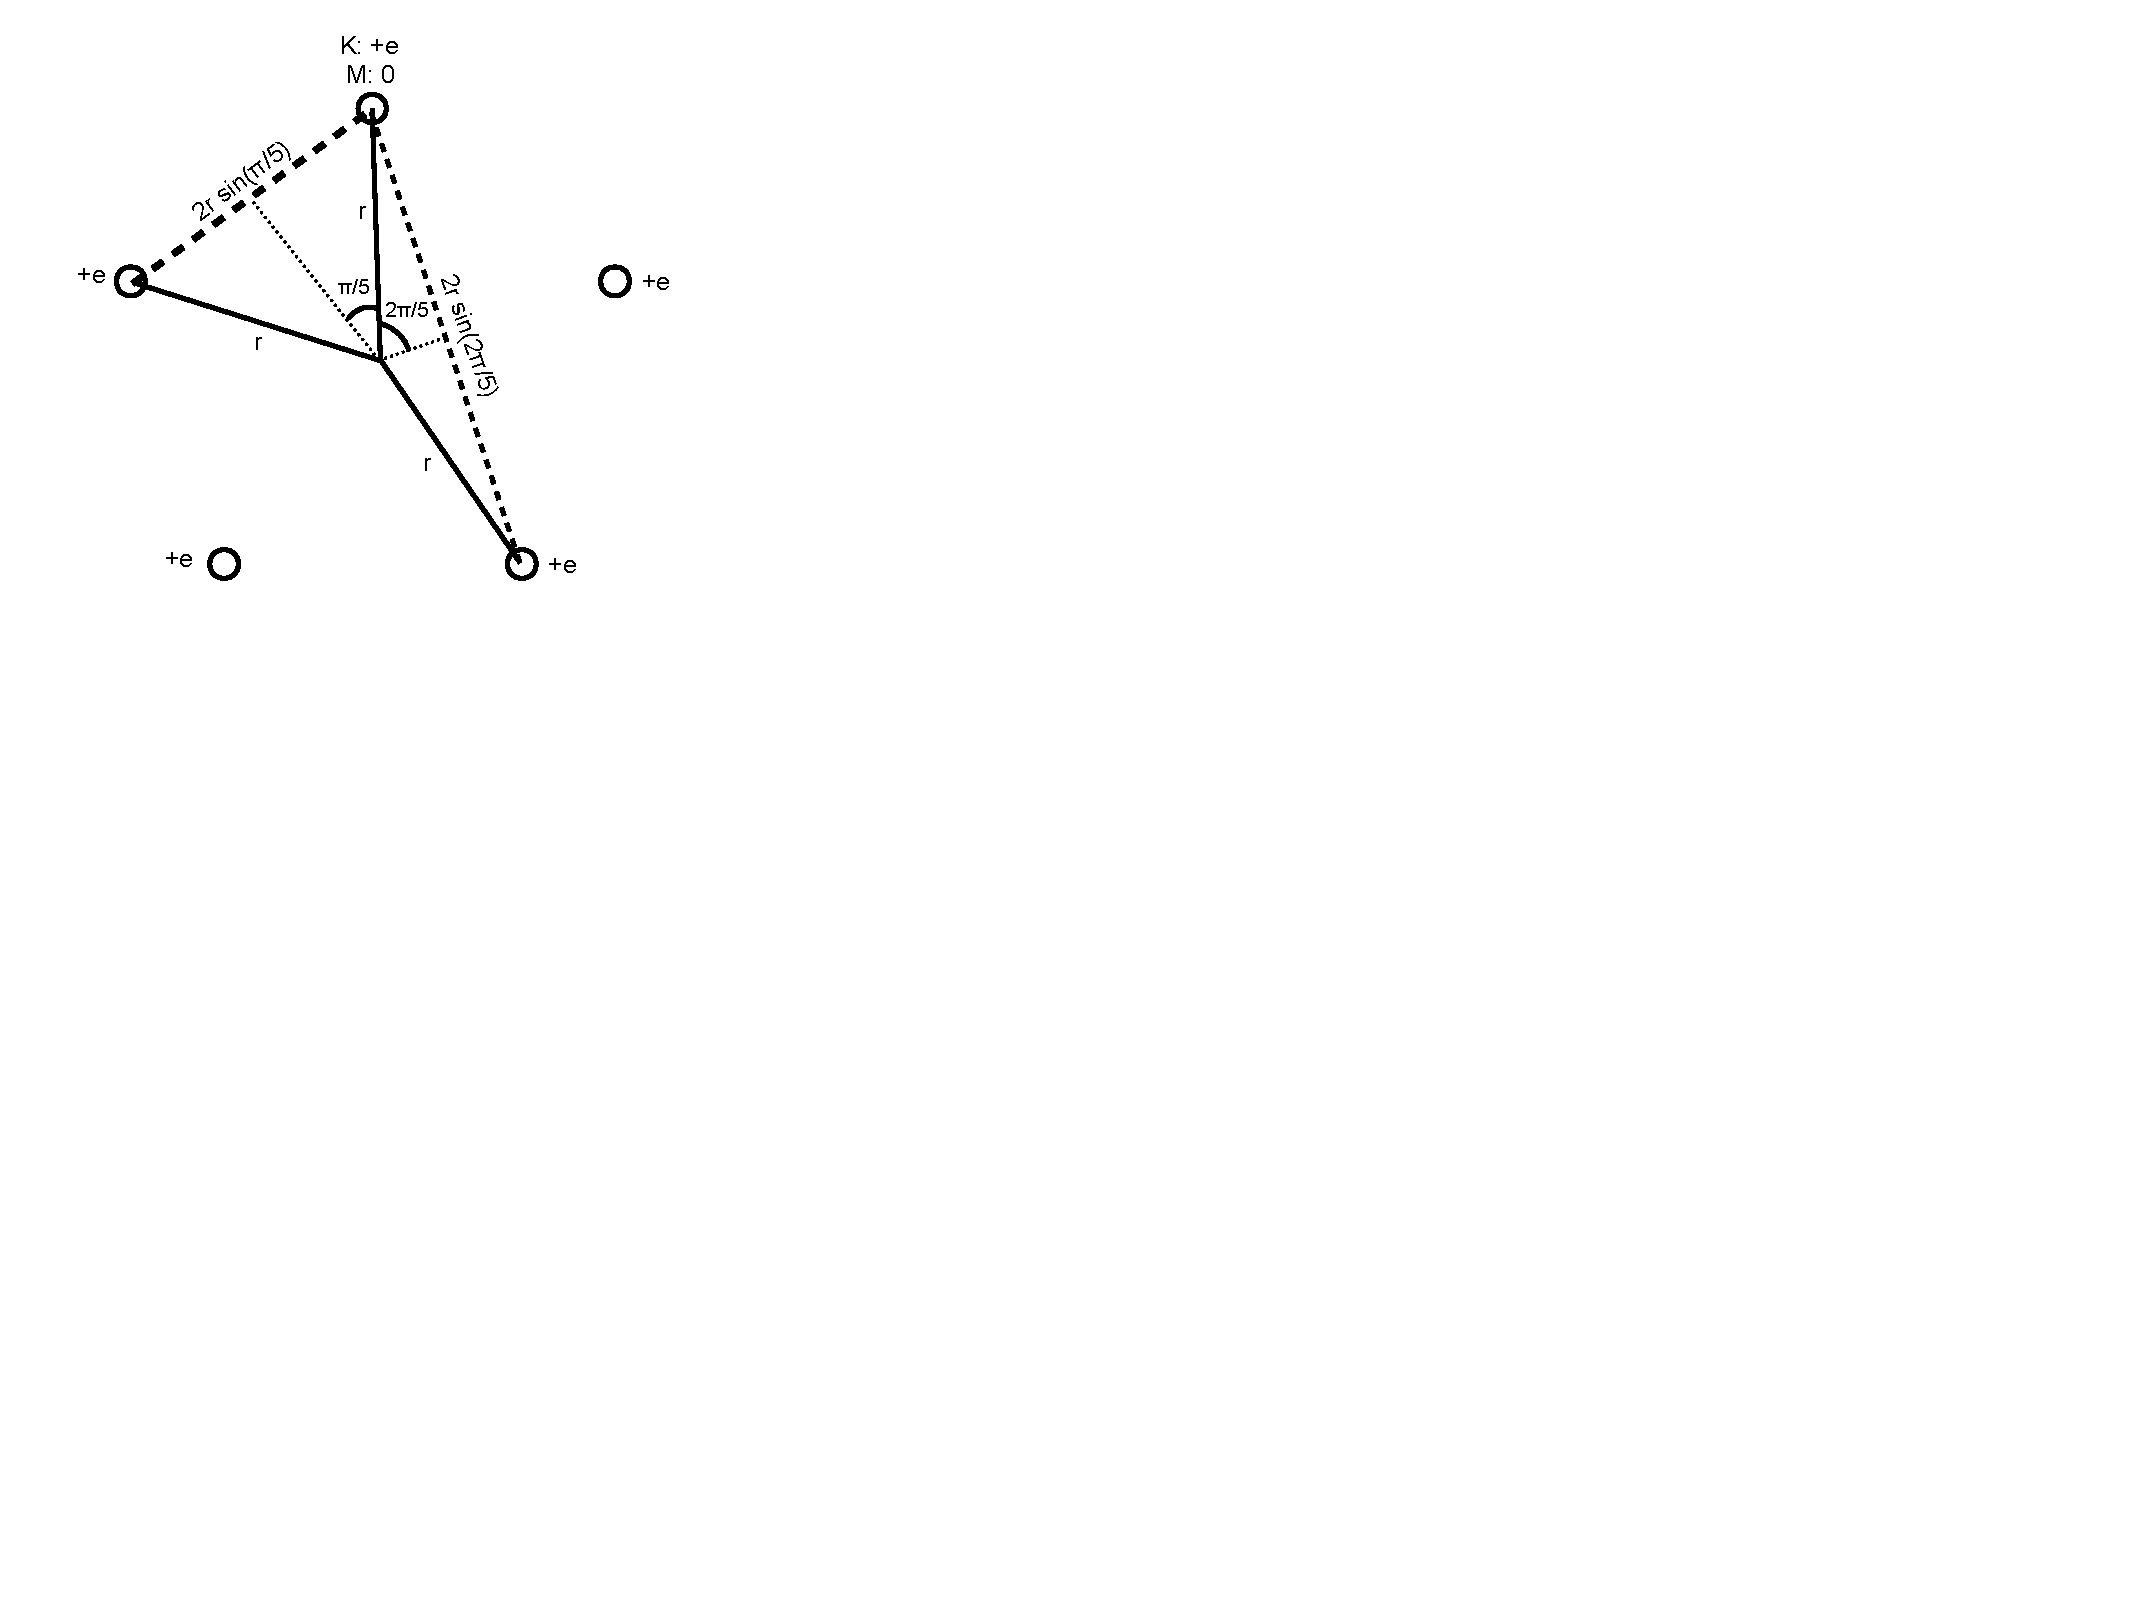
\includegraphics[height=2.5in]{figures/diagram.pdf}
\hspace{0.5in}
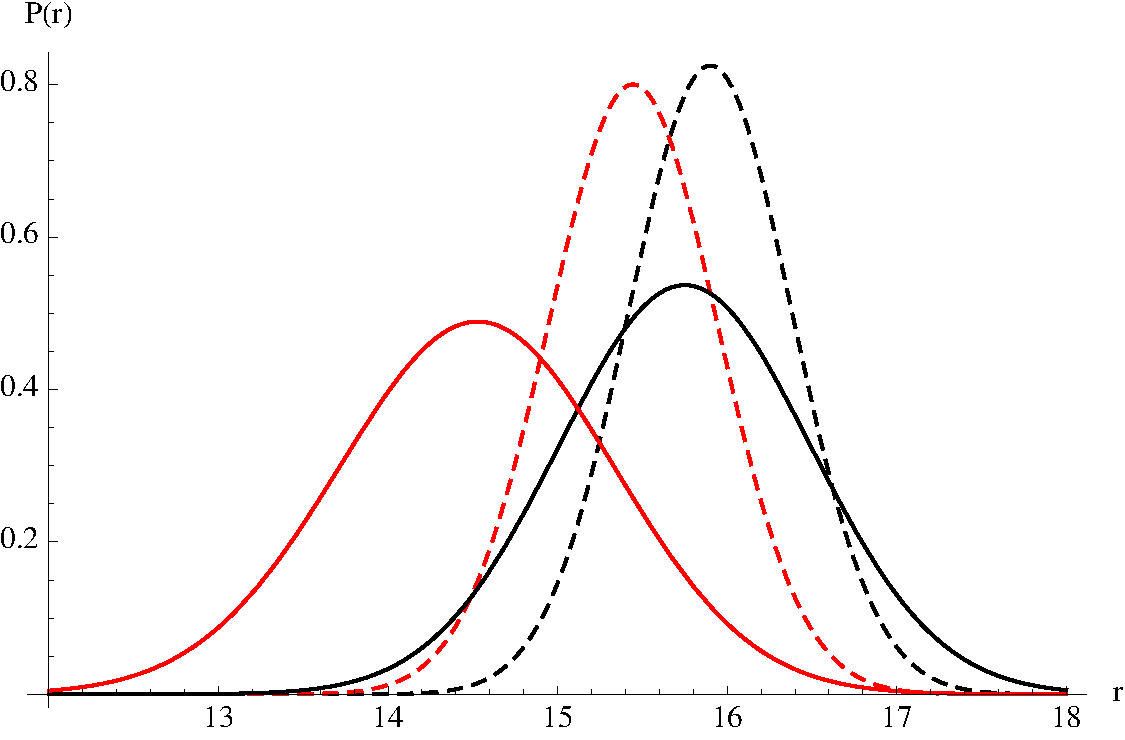
\includegraphics[height=2.2in]{figures/predict_distribution.pdf}
\caption{A) A conserved basic residue in the M2-M3 loop yields a pentamer of (un-screened) positive charges, which we refer to as the +5 ring,  corresponding to $\gamma$ K289, $\alpha$ K279, or $\beta$ K274.  The total energy of the +5 ring increases as the ring closes (and $r$ gets smaller), reducing/increasing the distance/repulsion between like-charges. The $\gamma$ K289M mutation neutralizes one of the charges, yielding a +4 ring, which can shrink with a lowered energetic cost.  B) (Placeholder) Predicted distribution  of $r$ generated using values in Table \ref{tab:prediction}; black is for a +5 ring (as in K289) while red is for a +4 ring (as in M289); dashed lines are for 300K and solid lines for 315 K.  
\label{fig:diagram}}
\end{center}
\end{figure}

\section{THEORY\label{sec:theory}}

The ring of five basic residues can be approximated as five positive charges arranged in a pentamer, each a distance $r$ from the center, which we refer to as the +5 ring.  The thermally excited ring may ``breathe'', causing $r$ to fluctuate, but for simplicity all charges are treated as equidistant from the center.   
The variation in $r$ is given by the time-average \begin{equation}
\varr = \langle (r(t) - \avgr)^{2}\rangle.  
\end{equation}  
At equilibrium, the wild-type receptor exhibits normal fluctuations of $r$ around its time average $\bar{r}$. The free energy of the wild-type receptor as a function of the +5 ring radius $r$ can be expanded harmonically as 
\begin{equation}
H_{K}(r) = \frac{k_{r}(r - \avgr_{K})^{2}}{2 \avgr_{K}},  
\end{equation}
where the time-average of $r$  is noted by $\avgr_{K}$, and $k_{r}$ is the temperature-dependent coefficient governing fluctuations: 
\begin{equation}
{k_{r} } = \frac{R T~\avgr_{K}}{ {\langle (r - \avgr_{K})^{2}\rangle}}, \label{eq:kr}
\end{equation}
where $R$ is the gas constant and $T$ is the temperature.  

The mutation $\gamma$K289M removes the four long-range repulsive electrostatic interactions involving $\gamma K289$.  Shrinking the pentameric ring is therefore less unfavorable in the presence of the mutation, and the free energy as a function of $r$ is reduced by the Coulomb energy of the lost interactions: 
\begin{equation}
\Delta U(r) =  \frac{ -k_{e} e^{2}}{r} \left(\frac{1}{\sin{2\pi/5}} + \frac{1}{\sin{\pi/5}}\right)  = - \frac{c k_{e}e^{2}}{r}
\end{equation}
where $c \sim 2.75$, $e$ is the electron charge, and $k_{e} = 332 \mathrm{\AA/kcal/mol}/e^{2}$ is the Coulomb constant. Note that this simplification is reasonable primarily because all five charges are nearly coplanar in a plane perpendicular to the pore axis.   Other electrostatic interactions will also be lost, but it is reasonable to neglect them because they involve residues screened by another oppositely charged residue, and/or they do not have a significant radial component.  
The total free energy for the mutant receptor is therefore 
\begin{eqnarray}
H_{M}(r) &=& H_{K}(r) + \Delta U(r) \\&=&  \frac{k_{r}(r - \avgr_{K})^{2}}{2 \avgr_{K}}- \frac{c k_{e}e^{2}}{r}%\\ 
\\&=&  k_{r}\avgr_{K}\left(\frac{(r - \avgr_{K})^{2}}{2 \avgr_{K}^{2}}  - \frac{\kappa { \avgr_{K}} }{{r}}\right), 
\end{eqnarray}
where 
\begin{equation}\kappa \equiv  \frac{c ~k_{e}e^{2}}{{k_{r} \avgr_{K}^{2}} }= \frac{c } {R T}\frac{k_{e}e^{2}}{\avgr_{K}} \frac{ \varr}{\avgr_{K}^{2}}\label{eq:kappadef} \end{equation}
The average radius for the mutant receptor, $\avgr_{M}$, minimizes $H_{M}$:
\begin{equation}
\left.\frac{\partial H_{M}(r) }{\partial r}\right|_{\avgr_{M}}= k_{r}\left(1 - \frac{\avgr_{M}}{\avgr_{K}} - \kappa \left(\frac{ { \avgr_{K}} }{\avgr_{M}}\right)^{2}\right) = 0.\label{eq:minimize}
\end{equation}
Defining the ratio between the two mean radii $\alpha \equiv \avgr_{M}/\avgr_{K}$, Equation \ref{eq:minimize} reduces to 
$1-\alpha- {\kappa}/{\alpha^{2}} =0.$
  ~This equation has an exact, real solution for $\kappa < 4/27$ ($\frac{k_{e}e^{2}}{k_{r} r_{K}^{2}}<0.035$), which when expanded around $\kappa = 0$ is 
\begin{eqnarray}
\alpha = \frac{\avgr_{M}}{\avgr_{K}}&=& 1 - \kappa - 2 \kappa^{2} - 7 \kappa^{3} + O(\kappa^{4}).
\end{eqnarray}
To first order in $\kappa$, we predict that 
\begin{equation}
\avgr_{M} = \avgr_{K} -  \frac{c k_{e}e^{2}} {R T}\frac{{ {\varr_{K}}}}{\avgr_{K}^{2}} \label{eq:predict}
\end{equation}
where $c k_{e} e^{2}/R= 8.3 \times 10^{5} ${ \AA} K.


\section*{RESULTS AND DISCUSSION}
\section*{Conformational Effects of Mutation}
\subsubsection*{+5 ring}

For comparison with the analytical model of the +5 ring presented in Theory,  the mean $\avgr_{K}$ and standard deviation  $ \sqrt{\varr_{K}} $ of the distance of +5 ring charges from the pore axis (see Figure \ref{fig:diagram})  were measured for the \WT systems at each temperature.  Results are in Table \ref{tab:prediction}, showing that $\avgr_{K}$ was not sensitive to temperature, while $\sqrt{\varr_{K}}$ increased with temperature, as expected.  These values, as well as Equations \ref{eq:kr} and \ref{eq:kappadef}, were used to calculate the parameters $k_{R}$ and $\kappa$ for each temperature.  

Eq. \ref{eq:predict} was used to generate predictions for $\avgr_{M}$, which were reduced relative to $\avgr_{K}$ at both temperatures, but with a much larger reduction at higher temperatures.  Quantitative agreement was very good, especially given the simplicity of the theory; at 300K we predicted a 3.1\% reduction upon mutation, but obtained a reduction of 2.5\%, while at 315K we predicted an 8.2\% reduction but obtained a 6.3\% reduction.  In both cases, the reduction was overestimated, which may reflect computational limits on equilibration time for the \MT receptor, or a higher order contribution to $H_{K}(r)$ resulting in a steeper free energy cost when $r-\avgr_{K}$ is large.     

\begin{table}[htp]
\caption{\label{tab:prediction} Observed values and extracted parameters from analysis of +5 ring in \WT receptors, and predicted and observed values upon mutating K289M (yielding +4 ring).}
\begin{center}
\begin{adjustbox}{width=0.5\textwidth}
\small
\begin{tabular}{|c|c|c|c|c|c|c|}
$T (K) $& $\avgr_{K} $(\AA) &$\avgr_{M}$(pred,\AA)&  $\avgr_{M}$(obs, \AA)& $ \sqrt{\varr_{K}} $ (\AA)& $\kappa$ & $k_{R}/\avgr_{K}$ (kcal/mol/\AA$^{2}$)\\
\hline
300 & 15.9 & 15.4 &  15.5 & 0.27 &  0.027&8.5 \\
315 & 15.8 &   14.5&  14.8& 0.42 &  0.066 &3.6
\end{tabular}
\end{adjustbox}
\end{center}
\label{default}
\end{table}%
\subsubsection*{Pore radius}

Although the simple electrostatic effects of neutralizing one charge in the +5 ring predict the observed closing of that ring, a functional effect requires that radius of the +5 ring is coupled to radius of the pore.  The pore radius profile (averaged across two replicas) for the \MT and \WT receptors is shown in Figure \ref{fig:pore-profile}.  The minimum constriction region (flanked by hydrophobic leucine residues) occurs at roughly the same height along the pore axis for the two systems, but is substantially tighter for the averaged mutant structure, particularly at higher temperatures.

 As shown in Figure \ref{fig:pore-evolution}, overlap between \MT and \WT trajectories (including individual replicas) is substantial at 300K, although the distribution of minimum pore radii is shifted slightly downward (smaller) for the mutant receptor. At 315K, this overlap is substantially reduced, with both \WT replicas yielding conformations with persistently larger pore radii than both \MT replicas. These trends mimic those observed in the +5 ring.  
 
Determining whether a single conformation corresponds to an ``open'' or ``closed'' state is not typically possible in MD simulations, but we note here that a Cl- atom has a radius of approximately 1.8\AA; at 300K,  the minimum pore radius is greater than 1.8\AA\ for 69\% (\WT) and 43\% (\MT) of the frames, while at 315K, the minimum pore radius is greater than 1.8\AA\ for 69\% (\WT) and 26\% (\MT) of the frames.  

All simulations here were done in the absence of GABA or other agonist, which is not stable in the agonist-binding site due to limitations of classical non-polarizable forcefields for capturing cation-$\pi$ interactions.  The presence of agonist would likely alter $\avgr_{K}$ and/or $k_{R}$, but would not affect $\Delta U(r)$, which depends only on protein sequence.  

%As shown in Figure \ref{fig:pore-evolution}, overlap between \MT and \WT trajectories (including individual replicas) is substantial at 300K, although the distribution of minimum pore radii is shifted slightly downward (smaller) for the mutant receptor. At 315K, this overlap is substantially reduced, with both \WT replicas yielding conformations with persistently larger pore radii than both \MT replicas. The difference in the distribution peaks between \MT and \WT is noticeably larger at 315K, reflecting the peak shifting  up (larger) for the \WT with increased temperature, and shifting in the opposite direction for the mutant.  A Cl- atom has a radius of approximately 1.8\AA; at 300K,  the minimum pore radius is greater than 1.8\AA\ for 69\% (\WT) and 42.5\% (\MT) of the frames, while at 315K, the minimum pore radius is greater than 1.8\AA\ for 68.9\% (\WT) and 26.3\% (\MT) of the frames. 

%The TMD consists of four helices(M1-M4) in each subunit and the M2 helices lines the pore. The pore radii of the channel measured using the HOLE software and scripting in VMD, has helped us understand the profile of the channel(Figure 2A). From  Figure 2B it is observed that the minimum constriction region is close to 2\AA , formed around 9' region (0\AA\ ) of the Z Axis.

%This minimum constriction region is flanked by hydrophobic LEU residues.With the radius of a chloride ion being 1.8\AA \cite{Shannon1976}, we understand that the wild-type receptor is just open enough to allow the ions through the channel. On comparison with the wild-type the minimum constriction region of the pore radii profile of the mutant falls below 1.8\AA\ thus blocking the channel for chloride ions. This difference between the Wild-Type and Mutant is even more conspicuous with the samples run at higher temperature(315K)(Figure 2B).Consequently the differences in the variations of the pore radii at the minimum constriction region is more evident at the higher temperature thus depicting the closure of the channel in the mutant(Figure 3). Figure 3 further substantiates the effect of temperature, as the probability distribution peak shifts to the left for the mutants while it remains the same for the wild-type, with the increase in temperature. Furthermore, the peak has broadened for the wild-type (as expected) with increase in temperature while this is not evident in the mutants. The increase in distance between the peaks(Figure 3B) of the mutant and wild-type and also the shift in the probability distribution peaks could be consistent with the flickering effect.

\begin{figure}
\begin{center}
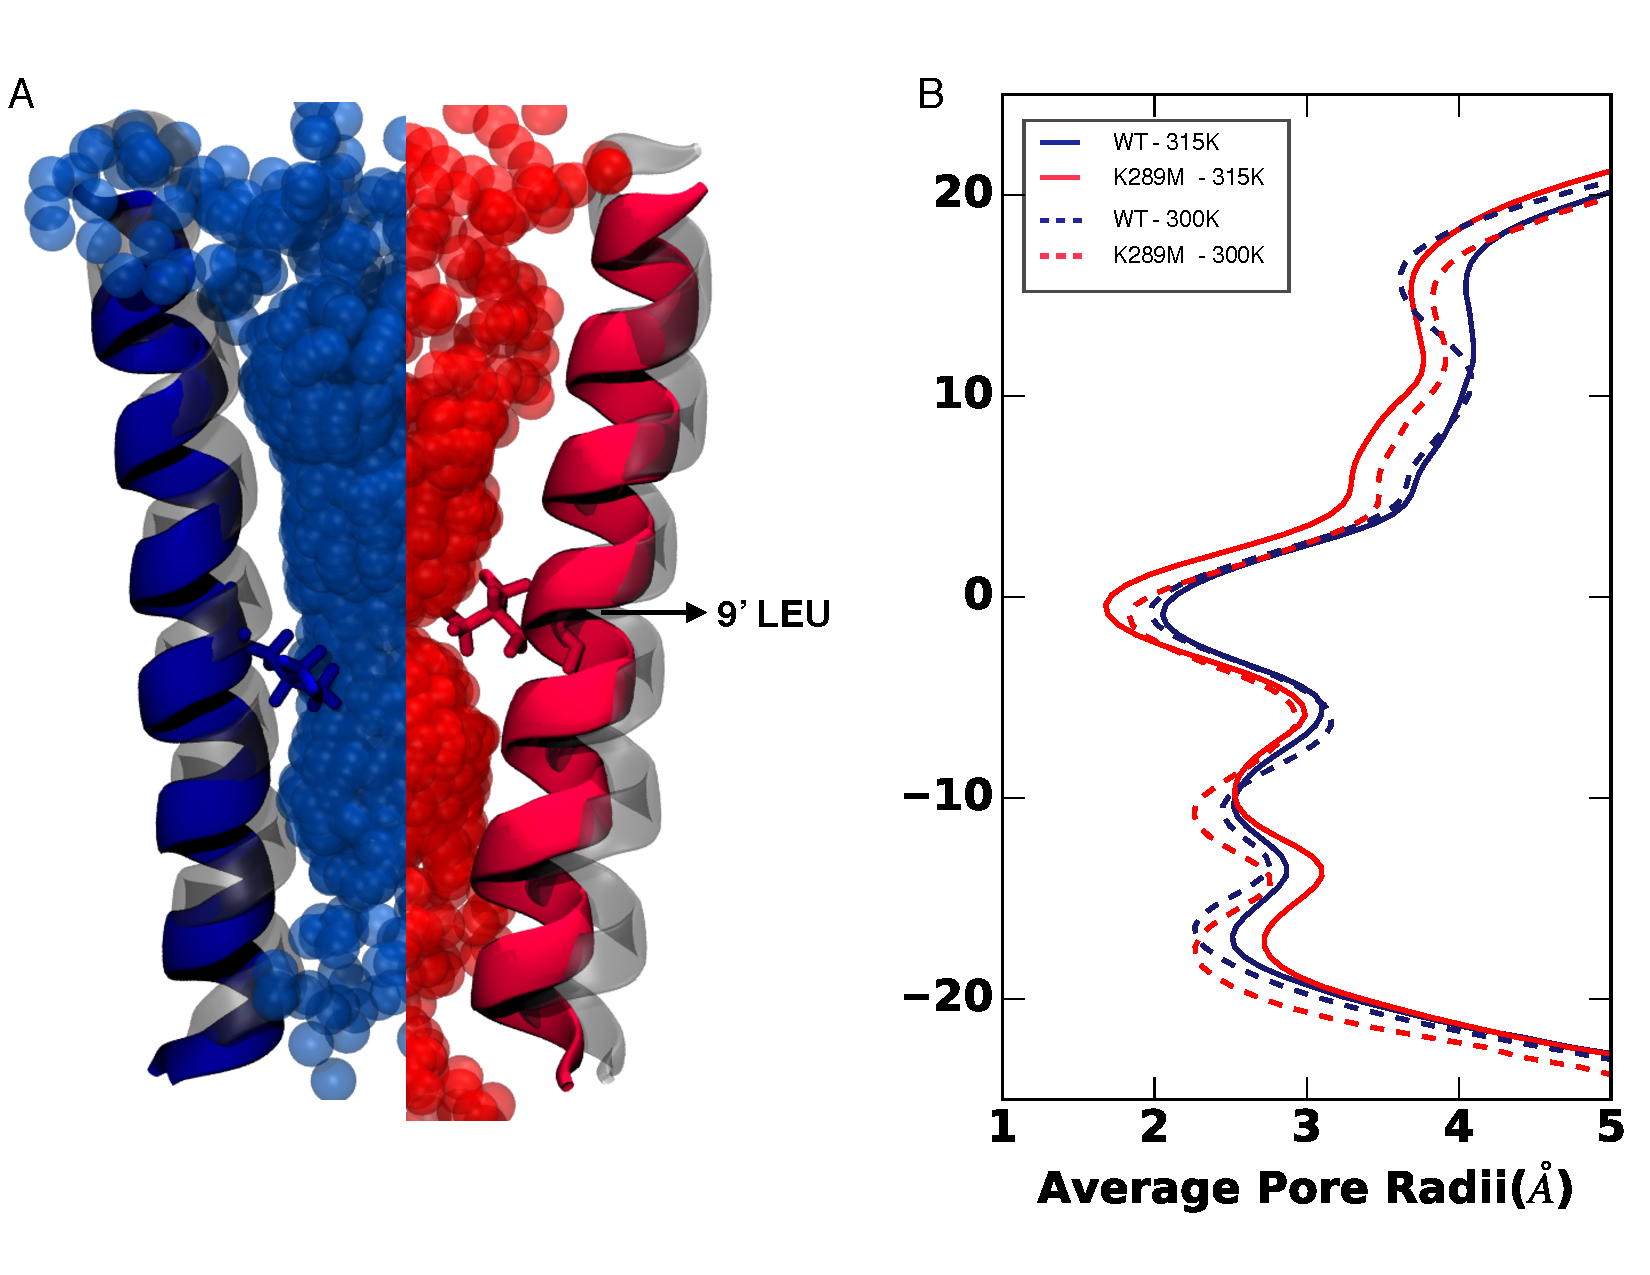
\includegraphics[width = .5\textwidth]{figures/pore_radd_fill.pdf}
\end{center}
\caption{(A) Space-filling models computed from simulations at 315 K, depicting the reduced pore radii of the \MT(red) as compared to that of the \WT(blue). (B) Radii of the transmembrane domain along the Z-axis, averaged over all the frames. The pore profile around the 9' region is more constricted at the higher temperature when compared to that of the lower temperature, in both the \WT and the \MT. The space filling models further compares the significant reduction in the pore radius in the \MT to the fairly open \WT, and the movement of helices compared to their respective initial conformations(gray).}
\label{fig:pore-profile}
\end{figure}

\begin{figure}
\begin{center}
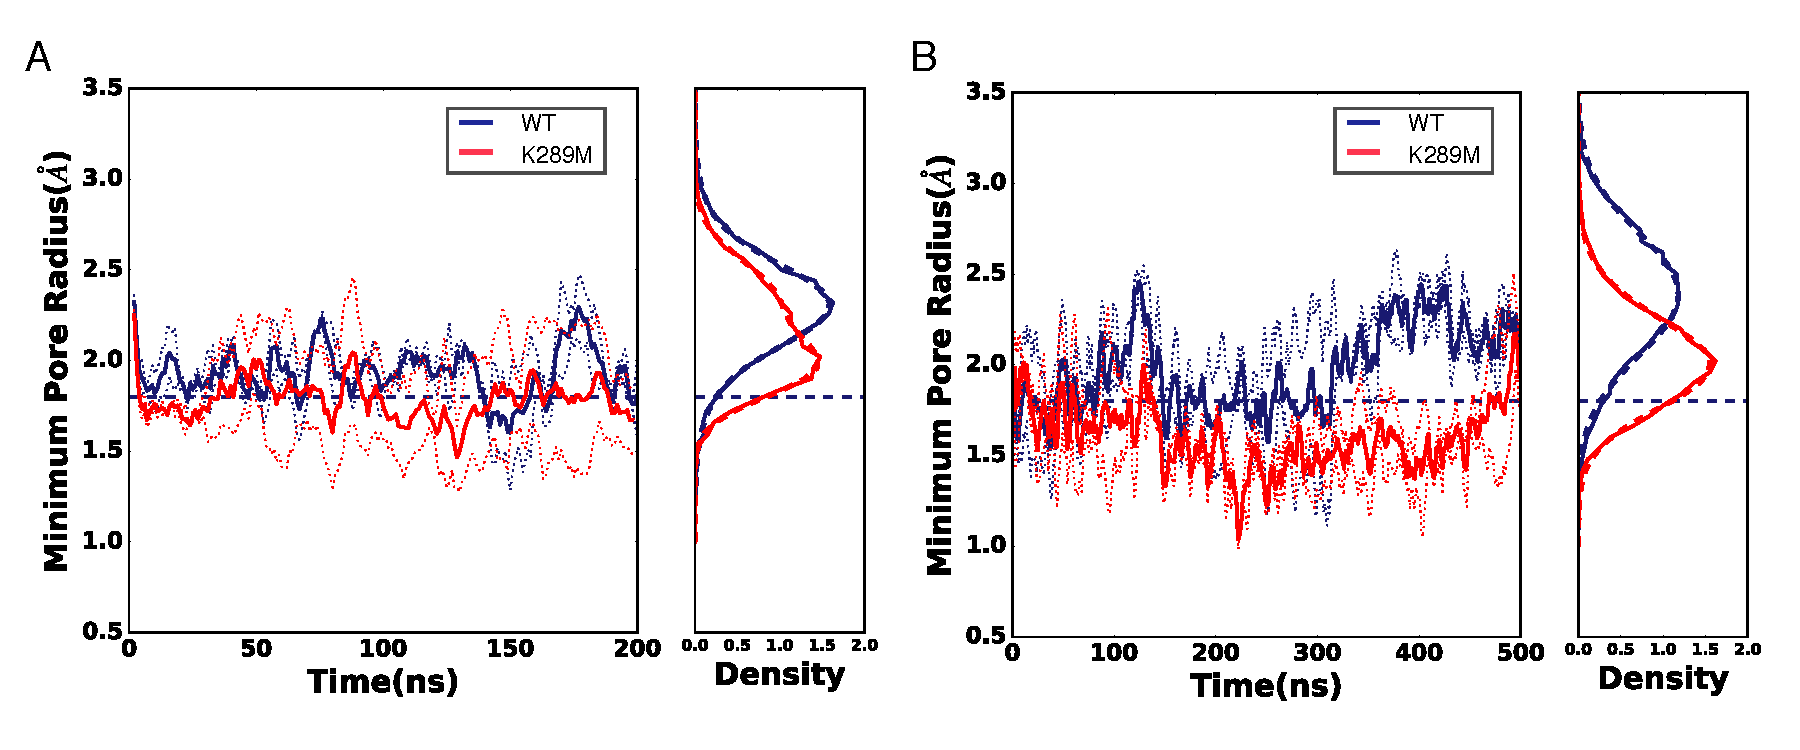
\includegraphics[width = .5\textwidth]{figures/min_pore_radd.pdf}
\end{center}
\caption{Smoothed time evolution of the pore minimum constriction, averaged (solid lines) over two replicas (dotted lines) each, at 300 K(A) and 315 K(B). The minimum constriction, formed around the 9' region is visibly more constricted for the \MTs and this reduction is more pronounced at higher temperature. The minimum constriction region in \MT falls below the chloride ion radius of 1.8\AA, thus driving it to a closed state. The probability distribution further shows a clear shift in the peak of the \MTs towards reduced pore radii at a higher temperature.}
\label{fig:pore-evolution}
\end{figure}

\subsubsection*{Drying of the pore}
To further understand the direct implication of the closing of the \MT channel, we measured the average number of water molecules in the pore channel. Many theoretical studies on water have shown that the interfacial drying can be caused by hydrophobic enclosures in the protein\cite{Zhu2010}. Furthermore, studies\cite{Zhu2012,Dong2013} have also shown that drying of the pore region could lead to blocking of the channel, since water is assumed to facilitate conduction of ions. As mentioned earlier, the pore facing residues in \GABAA are dominated by non-polar residues and this causes intermittent drying of the channel when the minimum constriction region comes closer to form hydrophobic enclosures. The plot (Figure \ref{fig:pore_water}A) shows the density of the water molecules throughout the simulation, along the Z-axis. The figure \ref{fig:pore_water}B further substantiates the plot by depicting the absence of water in the minimum constriction region of the pore, at higher temperature, in the \MTs . Thus, such dehydration of the channel could be a mechanism for inhibiting the conduction of the channel.

\begin{figure}
\begin{center}
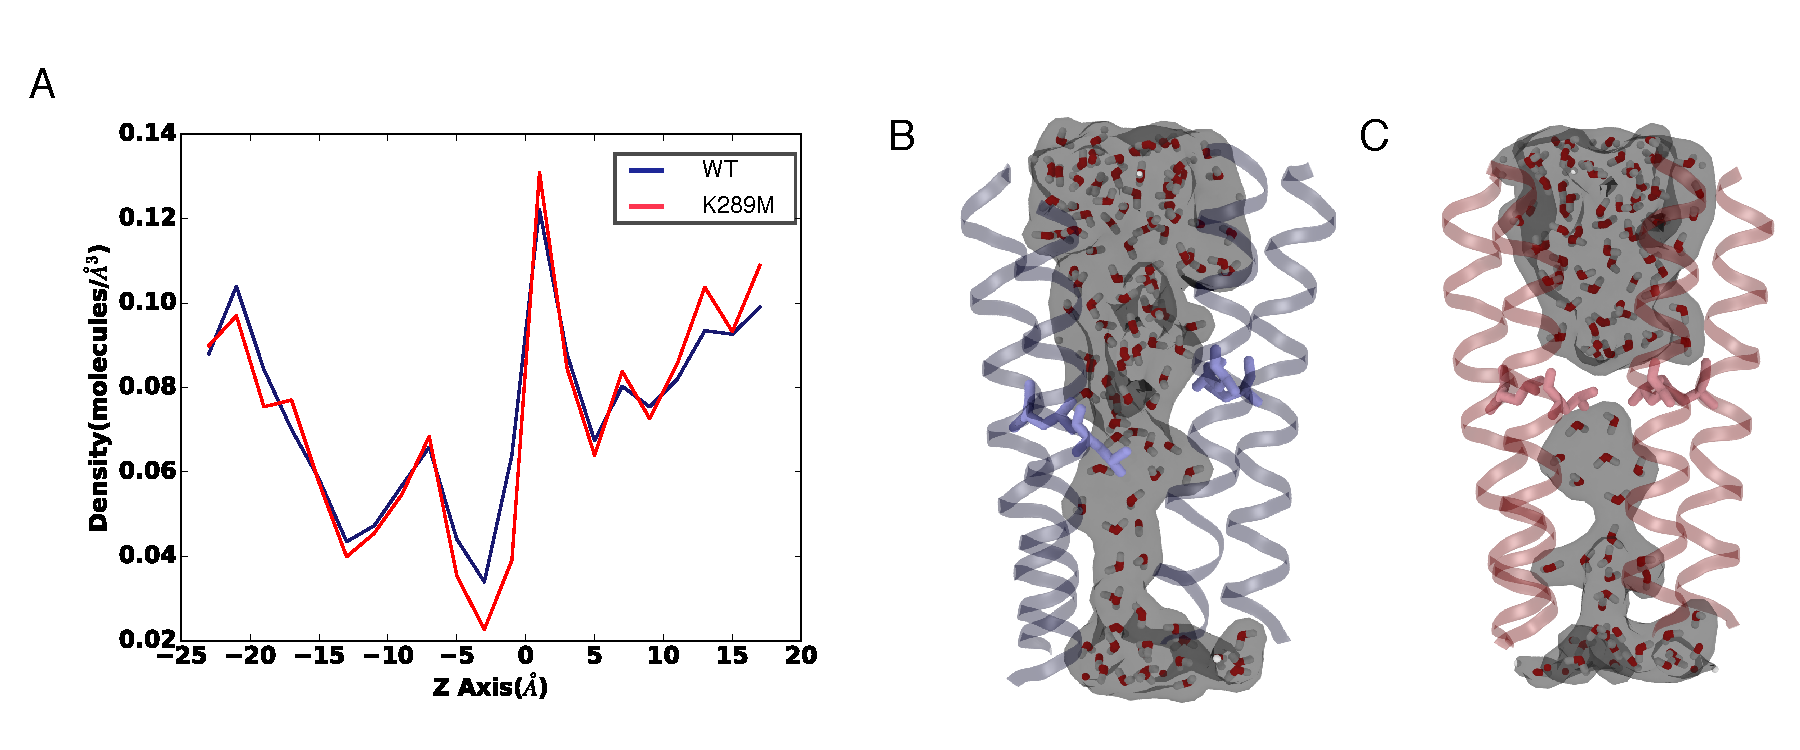
\includegraphics[width = .5\textwidth]{figures/water_pore.pdf}
\end{center}
\caption{(A)Number of water molecules along the Z-axis averaged over the frames and replicas. Presence of water in the constriction region of the \WT\ - M2 helices (B) as compared to the temporary dryness due to reduction in pore radii in the  \MT\ - M2 helices(C), at higher temperature. On an average, nearly zero no. of water molecules are found at the 9' region in the \MT\ system, depicting the stripping of water molecules due to the enclosure of the hydrophobic residues.}
\label{fig:pore_water}
\end{figure}

%\subsubsection*{Pentameric symmetry of M2 helices}
%
%
%\begin{figure}
%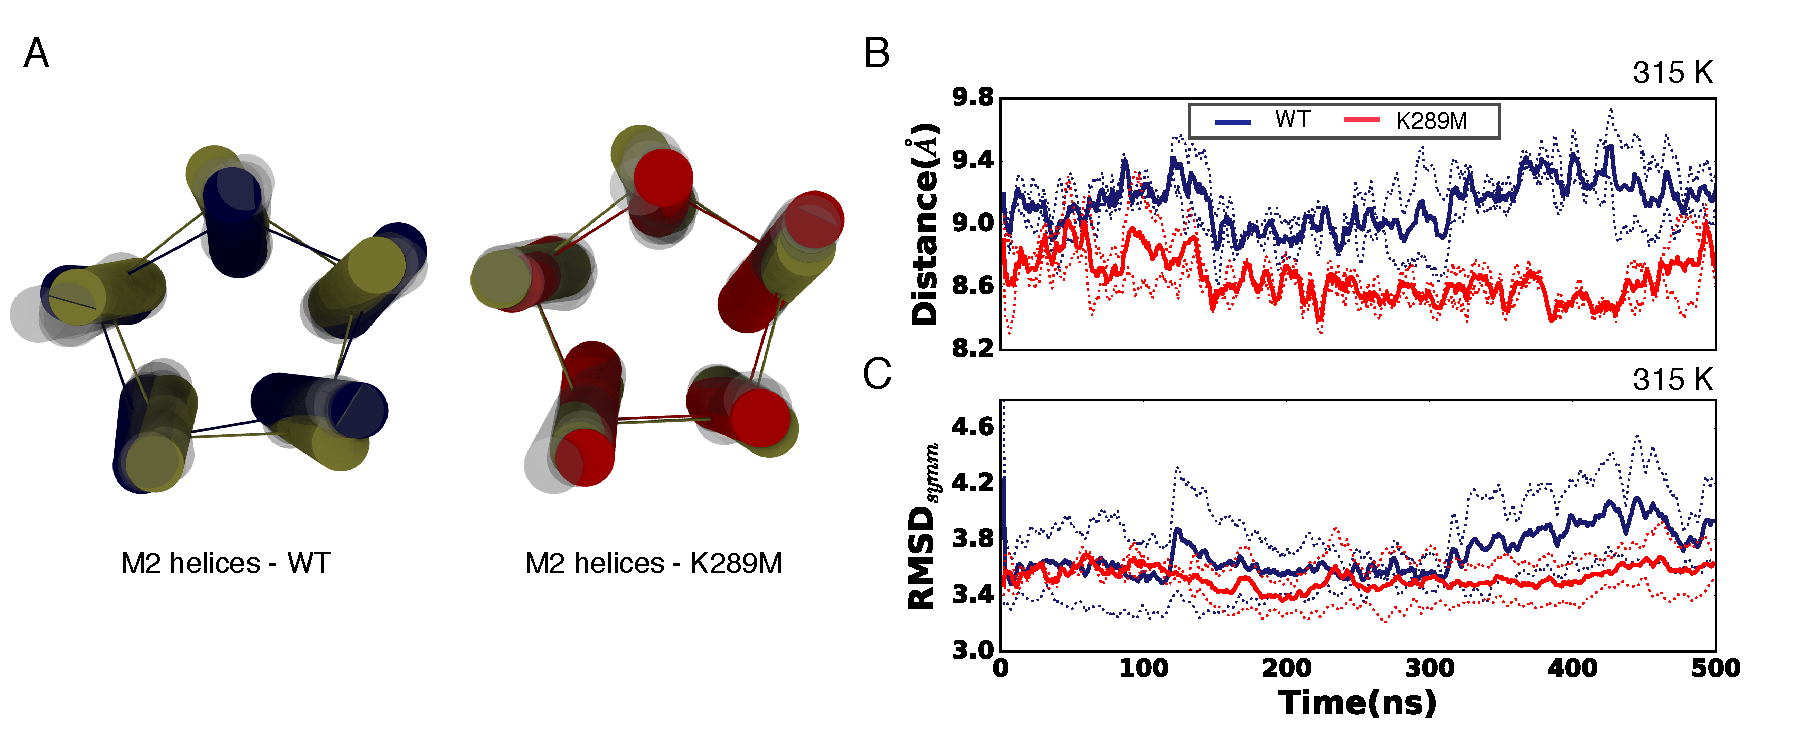
\includegraphics[width = 1\textwidth]{figures/pore_symm.pdf}
%\caption{(A) M2 helices conformation at every 100ns(gray) and at 500ns (Blue - \WT;Red- \MT).(B) Distances(solid lines) between the M2 helices averaged over two replicas(dotted lines) (315K).(C) Root mean square deviation of the symmetry of the M2 in each frame of its trajectory at 315K.}
%\label{fig:symmetry}
%\end{figure}
%
%In Figures \ref{fig:pore-profile} and \ref{fig:pore-evolution} we demonstrated that, particularly at higher temperatures, the mutant receptors favor conformations with tighter pore constrictions.  Visual observation indicated that, in general, the tighter \MT conformations reflected increased pentameric symmetry of the M2 helices (Figure \ref{fig:symmetry}).   We quantified this pentameric (a)symmetry using the symmetry \RMSD\ described in Methods, and found that at 315 K both \WT replicas had higher symmetry \RMSD\ (average: 3.80\AA) than both Mutant replicas (average: 3.54\AA) (Figure \ref{fig:symmetry} C).  The difference between the  \RMSD\ is $\approx$ 2.6\AA\ which follows a similar trend observed in open(symmetric) and closed(asymmetric) structures of GLIC with an \RMSD\ difference of 2.8\AA\ \cite{Zhu2010}. Such asymmetry for the \WT replicas is also reflected in the average distance between M2 helices, which is 9.13\AA\ for \WT and 8.65\AA\ for \MT (Figure \ref{fig:symmetry} B).  It should be noted that, in these simulations, wider pore radius was not associated with detectable differences in M2 helix tilt, but was most closely associated with lateral distance between the M2 helices.     
%%On analyzing the trajectory, we understood that the conformational changes in the pore occurs due to the individual movement of the M2/pore helices. The net effect of the tilts and twists of the pore helices throughout the simulation leads to an increased distance between the individual helices (Figure 5B) thus resulting in its loss of symmetry (Figure 5A) and openness of the pore in the wild-type. The mutant that tends to close during the course of the simulation seems to lack such drastic movements in the pore helices. This difference is substantiated by the highly varying RMSD of the wild-type pore helices compared to that of the constant RMSD of the Mutant (Figure 5B-below)).

\section*{Effects of Mutation on Conduction}
\subsubsection*{Electrostatic Barriers in the Channel}

The effects of the mutation on purely electrostatic barriers for chloride ion translocation was quantified via the Poisson-Boltzmann equation as described in Methods.  The mutation from a positively charged to neutral residue led to minute changes in the electrostatic profile given identical initial structures (as shown in Supplementary Figure S2(A) and Figure S2(B)), suggesting that the mutation alone could not affect conductance without any conformational changes. 
%However, these differences were very small compared to those observed (Figure S2(B)) after equilibration of the \WT and \MT receptors to the distinct conformations discussed in the previous section.  

The calculation performed on equilibrated  structures of \WT and \MT receptors showed a 5-10 kcal/mol (Figure S2(C)) higher electrostatic barrier in \MT , predominantly occurring in the transmembrane domain enclosing the residues containing the minimum pore constriction region. The LEU-gate constriction in addition to the loss of long range electrostatic interactions from K289 seems to contribute to the formation of higher barrier in the \MT.
We note that these calculations includes electrostatic contributions, but not van der Waals or entropic contributions; these terms are included in the measurement of the potential of mean force via Adaptive Biasing Force calculations as described subsequently. 


%The primary electrostatic barrier to conduction, in the pore of the channel, is about 2 kcal/mol  higher in the mutant receptor than the \WT. The absence of the residue K289's long range electrostatic effects on the entire pore of the channel(Supplementary Figure S1,S2) in addition to  the tighter constriction of the LEU residues seems to contribute to the formation of the higher barrier in the Mutant. We note that these calculations includes electrostatic contributions, but not van der Waals or entropic contributions; these terms are included in the measurement of the potential of mean force via Adaptive Biasing Force calculations as described subsequently.

%The primary electrostatic barrier to conduction, proximal to the leucine residues forming the tightest constriction, was about 2 kcal/mol  higher in the mutant receptor than the \WT. The absence of the residue K289's long range electrostatic effects on the entire pore of the channel(Supplementary Figure S1,S2) in addition to  the tighter constriction of the LEU residues seems to contribute to the formation of the primary barrier in the Mutant. A secondary barrier closer to the mutation (at z = 15 \AA) was also about 2 kcal/mol higher in the mutant receptors at both high and low temperatures than the equivalent barrier in the \WT at 300K; at 315K this secondary barrier nearly vanished for the \WT. The net attractive electrostatic effect influenced by residue K289 on the ion at the entrance of the pore,  as visualized from the SMD simulations (Supplementary Figure S5), contributes to the disappearance of the secondary barrier in the \WT. We note that these calculations includes electrostatic contributions, but not van der Waals or entropic contributions; these terms are included in the measurement of the potential of mean force via Adaptive Biasing Force calculations as described subsequently. 

%To interpret the effects of the above mentioned conformational changes on the conductance of the channel, we performed some implicit solvent calculations.Since the mutation involves a charged residue, it is reasonable to assume that it might influence the electrostatic barriers of the channel. This led us to obtain the Poisson-Boltzmann(PB)\cite{Fogo2002} electrostatic potential profile of the channel. This calculation, performed using APBS1.3\cite{Baker2001}, gives us an idea about the electrostatic environment encountered by an ion as it travels through the channel.

%The electrostatic interactions are long range interactions and thus are expected to have a significant effect throughout the channel. Figure 6 represents the PB profile of the translocation of chloride ion through the channel. It depicts the PB profile of the channel (TM domain) for Cl- ion, at lower and higher temperature after equilibration of 200 ns and 400ns respectively. The mutants showed significantly higher barriers at these regions. The lysine(K289) residue in the wild-type, being a positively charged residue at the entrance of pore, could have created a favor- able environment for the negatively charged ion to pass through and this in turn could have reduced the barriers; however this effect is only visible after the equilibration. This result can further be substantiated by calculating the free energy changes as the ion passes through the channel along the Z-axis, which will include van der waals and entropic terms.

\begin{figure}
%\begin{center}
\centering
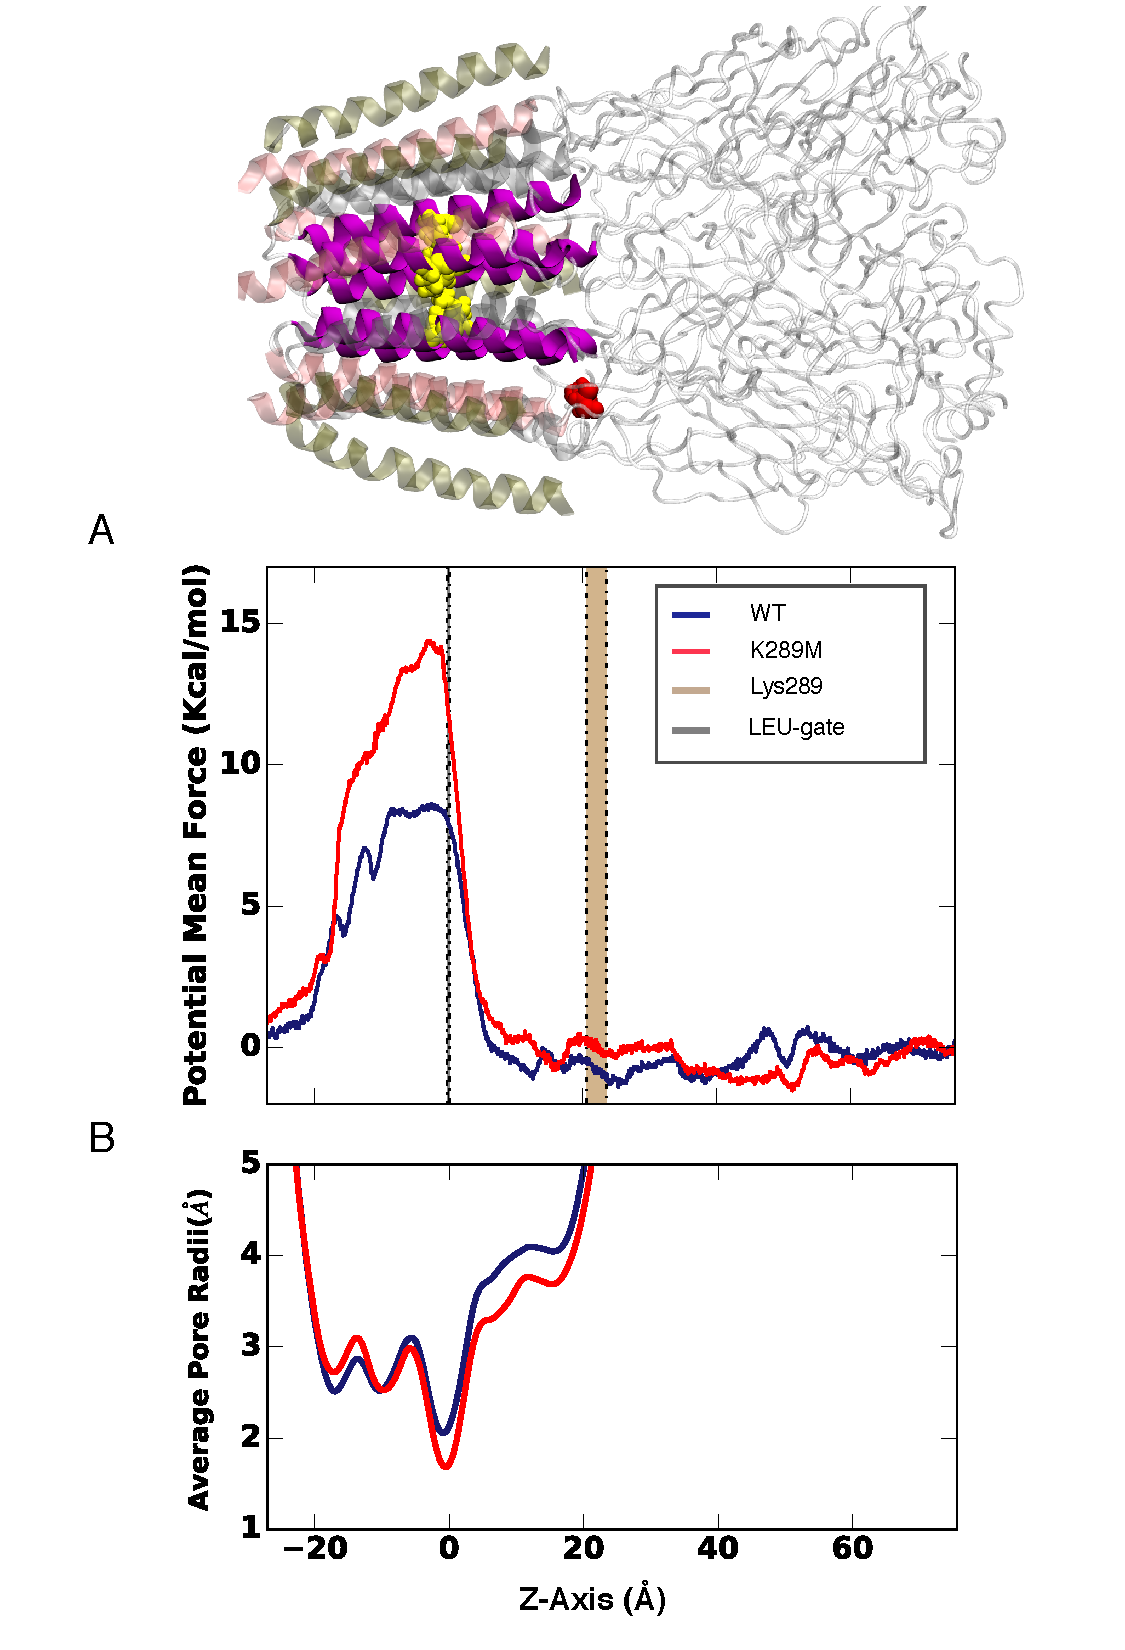
\includegraphics[width = .5\textwidth]{figures/ABF_pic_2.pdf}
\caption{ Potential of mean force profile of chloride ion transport  (A) Aligned below the horizontally laid protein figure is the plot showing the potential mean force experienced by the ion as it moves through the channel along the Z-axis. (B) These barriers in the channel are further compared with the average pore radius of the TM region of the channel. These comparisons clearly explains that the highest barriers are found at the 9' regions which forms the minimum constriction region. The difference between the barriers at this region is approximately 5 Kcal/mol.}
\label{fig:abf}
%\end{center}
\end{figure}

\subsubsection*{Potential of Mean Force}

The PMF for chloride ion translocation at 315K, measured using ABF, is shown in Figure \ref{fig:abf}. The largest barrier occurs more proximal to the leucine residues forming the tightest constriction; this barrier is increased by 5 kcal/mol for the mutant receptors. 
%The secondary electrostatic barrier closer to the mutation in Figure S5 is not clearly reflected in the PMF.  
A slight, broad well (relative to a reference position outside the receptor) is apparent around residue 289 in the PMF for the \WT receptor, while at the same location in the \MT receptor the PMF is slightly elevated relative to the reference location.  However, these differences are slight compared to the effects of the mutation on the primary barrier, indicating that while mutation of a positively charged to neutral residue does have a small effect on affinity of the chloride ion for the region of the receptor near the mutation, the dominant effect of the mutation on conduction is via conformational instability of the open state. 
%To calculate the free energy changes along a reaction coordinate, the potential mean force (PMF) is to be calculated. We undertook steered molecular dynamics(SMD) followed by Adaptive biasing force(ABF) methods to obtain PMF from the MD simulations. The average force experienced by the ion as a function of position in the channel displays the barriers experienced by the ion along the Z-Axis (Figure S1). Favorable positions of the ion along the channel, initially identified by performing SMD simulations, were used as the initial structures to perform simulations using ABF.

%The average force experienced by the ion as a function of position in the channel displays the barriers experienced by the ion along the Z-Axis. 
%This result coincides with the previous results by conveying that the mutant experiences higher force at the minimum constriction region as compared to the wild-type.(Figure 5 (left))

%The PMF plot obtained after the convergence of the forces, shows the free energy barriers along the channel, after sufficient sampling of the reaction coordinate (Figure 7B). On comparison with Figure 7C), it is evident that barriers in the channel coincide with the profile of the channel. It is therefore conclusive that the highest energy barrier is around the region flanked by the leusine residues, depicting the gating region of the channel.  Further, the effect of mutation along with the elevated temperature has increased the energy barrier by ~5 Kcal/mol, thus portraying the influence of the mutation in causing febrile seizures.

%\cleardoublepage

\section*{CONCLUSION}

Proteins that require ligand-induced conformational change have an inherent design challenge.  Free energy differences between conformations must change sign upon ligand binding, constraining the magnitude of this free energy difference in either the bound or apo state.  This behavior must still be robust to temperature variations experienced within the organism.   Although that temperature range is relatively narrow for endothermic animals,  it includes elevated temperatures for fighting infection. Differences in body temperature among endothermic species % (partially to satisfy different metabolic requirements \cite{ClarkeRothery}) 
may also drive some sequence differences in non-metabolic proteins. 

In this work, we investigated the effects of a fever-associated charged-to-hydrophobic mutation in a human ligand-gated ion channel, allowing us to identify the significance of collective, long-range, electrostatic interactions for maintaining the protein's function at higher temperatures.  The temperature-dependent structural effect of reducing these electrostatic interactions via substitution of K to M at  $\gamma2$: M2 $24^{\prime}$ can be well-predicted simply by considering Coulombic repulsions between charged residues at M2 24$^{\prime}$ in all subunits, as well as a simple variational theory which introduces temperature effects.  The phenomenon of unstable activation in $\gamma2$ K289M \GABAA,  previously observed {\it in vivo} and {\it in vitro}, has now been observed {\it in silico} and {\it in principio}.  

A basic residue at 24$^{\prime}$ in the M2-M3 loop is highly conserved across \GABAA subunits,  but not across all \plgics.  It is not necessary, however, that charged residues be positioned at 24$^{\prime}$ for cross-pore repulsions to stabilize open conformations, but simply that they be in the same position in each subunit.  Crucial collective interactions might therefore be well indicated by the presence of a charged residue that appears at the same position in all pore-sharing species (i.e. all \GABAA subunits or all GlyR subunits), but which is non-conserved across \plgics ~in general. 
 
To maintain the necessary range for cross-pore interactions, it is critical that the charged residues be  unscreened.   Presence of a nearby oppositely charged residue in one subunit will reduce the charge-charge interaction ($1/r$) to a charge-dipole interaction ($1/r^{2}$), with presence of an additional charged residue on the other side yielding a dipole-dipole interaction ($1/r^{3}$).  Screening may be affected by changes in pH as well as participation in salt-bridges, suggesting a mechanism that may be crucial for gating in numerous other \plgics.  Based on these results and those in Ref. \cite{Kash2003}, we suggest that $\alpha$D57 or $\alpha$D14 may screen $\alpha$K279 (M2 24$^{\prime}$) in the apo state, while binding of GABA changes conformation of $\alpha$D57 or $\alpha$D14,  leaving $\alpha$K279 (M2 24$^{\prime}$) unscreened, increasing cross-pore repulsions among positively charged residues at M2 24$^{\prime}$, and opening the pore.  

%Furthermore, these interactions will be most influential when all five subunits have the unscreened charged residue in the same position.  Crucial collective interactions might therefore be indicated by the presence of a charged residue that appears at the same position in all pore-sharing species (i.e. all \GABAA subunits). Non-conservation across other $\plgics$ (i.e. GluCl)  would actually be consistent with a significant role in \GABAA cross-pore interactions, because GluCl and \GABAA subunits do not share a pore.  

%In this work, we investigate the effects of the disease-associated K289M mutation in the $\gamma_2$ subunit of the \GABAA on conformation of the ion channel pore as well as free energy barriers for ion conduction.  The K289M mutation is associated with seizures caused by fever; after running simulations at two temperatures (300K and 315K) we observed that an increase in temperature had opposite effects on the pore radius in the \WT and K289M mutants, across multiple replicas.  As a result, conformational differences that were relatively slight at lower temperature were amplified significantly at higher temperature, even across multiple replicas.  When simulated at higher temperature, the K289M mutant was more likely to adopt a pore conformation with reduced pore radius, which is consistent with loss of \GABAA function at higher temperatures and subsequent seizures.  Measurement of the PMF of ion translocation confirmed that the reduced constriction increased the barrier to translocation by 5 kcal/mol.  %How does this relate to 10 kcal/mol WT? is WT conducting?
%  
%Several remarks should be made concerning the conditions of the simulations reported here.  First, 300K is certainly lower than normal body temperature, and 315K corresponds to a fever on the extreme high end of survivability.  The larger temperature difference was used to amplify signal in the simulations; such effects can be extremely challenging to extract from simulations conducted under very similar conditions due to computational limitations on simulation length and number of replicas. Our interpretation of the results therefore relies on the assumption that the effect of temperature on pore radius exhibits a relatively simple, monotonic trend over the 300-315K range.  
%
%Second, it has been frequently challenging to draw correspondence between the functional state of a pLGIC and the conformation represented in crystal structures.  The \GABAA model used in the present study is based on a structure of GluCl with agonist (ivermectin) bound to the intersubunit sites in the transmembrane domain and a pore sufficiently large for conducting ions, and consequently has typically been interpreted as being in an activated state.  In our \GABAA model, the ivermectin has been removed (and no agonist is bound to the orthosteric site); however, the presence of cholesterol lodged in the intersubunit site appears to stabilize a relatively open pore (minimum constriction of approximately 2\AA) over the course of 200 ns simulations. 



%Crystal structures of channels that are in an open state are GluCl(3RHW) which has a minimum pore constriction of  \(\approx\)2.3\AA\cite{Hibbs2011} and GLIC(3EAM) which has a pore that narrows down to a radius of 2.5\AA\cite{Bocquet2009}. While the  crystal structures in the non-conducting state are the \GABAA - (4COF)\cite{Miller2014a} which has a pore radii of  \(\approx\)1.575\AA\ and ELIC(2VL0)\cite{Hilf2008a} has a pore radii of \(\approx\)1\AA\ .
 
 %%GABAAr alpha ----  GluCL alpha = 36.8% identity
 %%			     ------  GABABeta = 41.6% identity
 
 %%GABAAr gamma ----  GluCL alpha = 33.2% identity
 %%			     ------  GABABeta = 44.6 % identity
 
 
 
  %We have visualized the effects of the mutant K289M on the conformation and conduction of the receptors by analyzing the trajectories and running free energy calculations.

%Simulations were performed with two replicas of the WT and Mutant and the conformational changes observed are a result of the average of the effects observed in the individual simulations. Further these results were compared with the results obtained from a similar set of simulations run at higher temperature(315 K).Realizing the exacerbated effects of the temperature on the mutants, the free energy calculations were run on one of the replicas at higher temperature. 

%1. In accordance to the previously done experimental studies\cite{Bianchi2002}, the reduction in the mean of the pore radii was observed in the mutants.

%2. The reduction in pore radii at the minimum constriction region flanked by the LEU residues confirms the presence of a hydrophobic gate, as suggested in a close homologue of GABA\textsubscript{A} receptor, GLIC \cite{Zhu2012}.

%3. Further this minimum constriction around the hydrophobic region is followed by drying of the channel in that region, in the mutants.

%4. Implicit solvent calculations , gave us a rough idea of high the energy barriers at the hydrophobic gate region in the mutants , as compared to a lower barrier in the wild-type.

%5. The explicit ABF free energy calculations, depicted the exact channel barriers and also the effects of the mutation on gating of the channel.

%6. One possible mechanism used by the WT to open could be by increasing the distance between M2 helices and thus losing the symmetry of the pore (Figure 4).

%7. This loss of symmetry could be initiated by the electrostatic effects of the charged K289 residue that is absent in the Mutant.


\section*{SUPPLEMENTARY MATERIAL}

%\ack{An online supplement to this article can be found by visiting BJ Online at http://www.biophysj.org.}\vspace*{-3pt}





\cleardoublepage
%\bibliographystyle{ieeetr}
\bibliography{GABAa_K289M}
\end{document}
